\chapter{Understanding Change Over Time – Change and Motion}

\section{Introduction}
Calculus is the branch of mathematics that focuses on change. While algebra helps us solve for unknown values and geometry deals with shapes and spaces, calculus answers questions about how things change over time, how fast things move, or how quantities accumulate.

Don’t let the idea of calculus intimidate you! At its core, calculus is simply a way of understanding rates of change and accumulation. Whether it’s predicting the speed of a car, calculating areas under curves, or modeling population growth, calculus provides the tools to solve these kinds of problems.

In this chapter, we’ll explore the basics of derivatives and integrals, the two main concepts of calculus, and how they help us describe change and motion.

\section{What Is a Derivative?}
A derivative tells us how a function is changing at any given point. It measures the rate of change or the slope of a curve at a specific point. In simpler terms, it answers questions like:
\begin{itemize}
    \item How fast is a car moving at a specific moment?
    \item How quickly is the population growing?
\end{itemize}

\subsection{The Concept of Slope}
In algebra, the slope of a line is a measure of its steepness, and it tells us how fast one variable changes with respect to another. In calculus, the slope is used to describe the instantaneous rate of change of a function.

\subsection{Example}

For a linear function like \( f(x) = 2x + 3 \), the slope is constant. The derivative of this function is 2, meaning the rate of change is the same no matter where you are on the line.

\begin{center}
    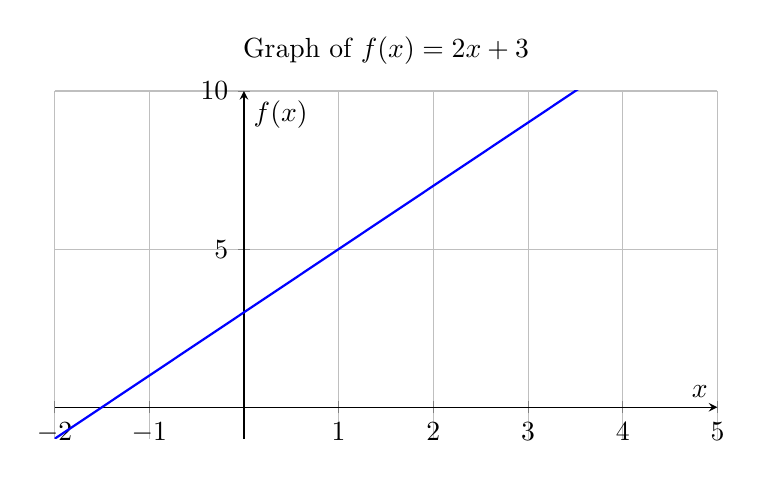
\begin{tikzpicture}
        \begin{axis}[
            axis lines = middle,
            xlabel = \(x\),
            ylabel = {\(f(x)\)},
            ymin=-1, ymax=10,
            xmin=-2, xmax=5,
            grid = major,
            width=10cm,
            height=6cm,
            domain=-2:5,
            samples=100,
            title={Graph of \( f(x) = 2x + 3 \)}
        ]
        \addplot[blue, thick] {2*x + 3};
    \end{axis}
    \end{tikzpicture}
    \captionof{figure}{Graph of the linear function \( f(x) = 2x + 3 \). The slope is constant across the entire line.}
\end{center}

But what happens when the function isn’t a straight line? For functions that curve, like \( f(x) = x^2 \), the slope (or rate of change) varies depending on the point. The derivative helps us figure out the slope at any point along the curve.

\begin{center}
    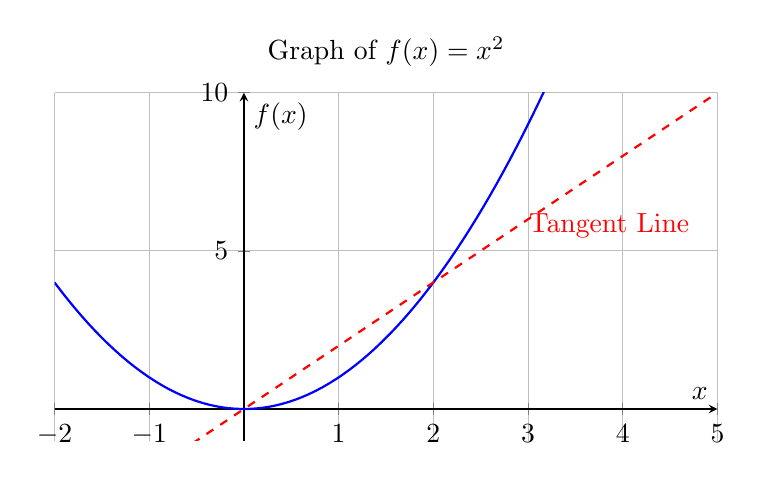
\begin{tikzpicture}
        \begin{axis}[
            axis lines = middle,
            xlabel = \(x\),
            ylabel = {\(f(x)\)},
            ymin=-1, ymax=10,
            xmin=-2, xmax=5,
            grid = major,
            width=10cm,
            height=6cm,
            domain=-2:5,
            samples=100,
            title={Graph of \( f(x) = x^2 \)}
        ]
        \addplot[blue, thick] {x^2};
        \addplot[red, dashed, thick, domain=-2:5] {2*x} node [pos=0.7, right] {Tangent Line};
    \end{axis}
    \end{tikzpicture}
    \captionof{figure}{Graph of the quadratic function \( f(x) = x^2 \). The red dashed line shows a tangent at a point, illustrating the slope at that specific point.}
\end{center}

\section{Finding Derivatives}

The derivative of a function is found using rules that make the process easier. These rules simplify how we calculate the rate of change for different types of functions.

\begin{itemize}
    \item \textbf{Power Rule:} If \( f(x) = x^n \), then the derivative is \( f'(x) = nx^{n-1} \).
    \item \textbf{Constant Rule:} The derivative of a constant function is zero.
    \item \textbf{Sum Rule:} The derivative of the sum of functions is the sum of their derivatives.
    \item \textbf{Product Rule:} If \( f(x) = g(x) \cdot h(x) \), then the derivative is \( f'(x) = g'(x)h(x) + g(x)h'(x) \).
    \item \textbf{Quotient Rule:} If \( f(x) = \frac{g(x)}{h(x)} \), then the derivative is:
    \[
    f'(x) = \frac{g'(x)h(x) - g(x)h'(x)}{h(x)^2}
    \]
    \item \textbf{Chain Rule:} If \( f(x) = g(h(x)) \), then the derivative is \( f'(x) = g'(h(x)) \cdot h'(x) \).
\end{itemize}
\begin{itemize}
    \item \textbf{Power Rule:} If \( f(x) = x^n \), then the derivative is \( f'(x) = nx^{n-1} \).
    \begin{center}
        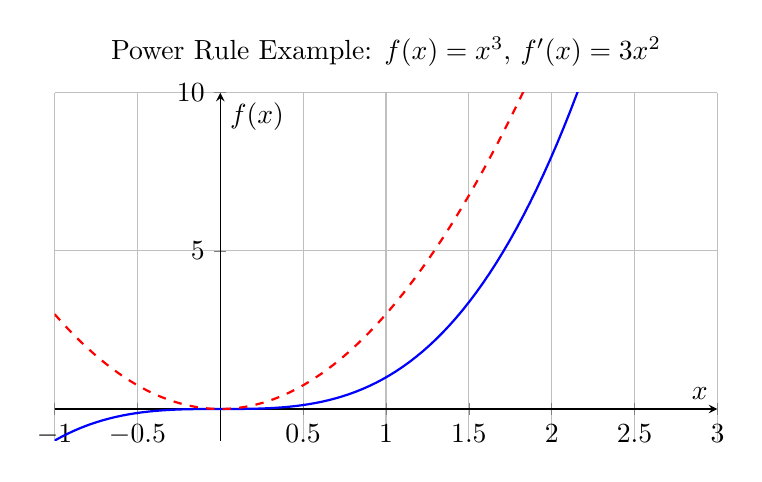
\begin{tikzpicture}
            \begin{axis}[
                axis lines = middle,
                xlabel = \(x\),
                ylabel = {\(f(x)\)},
                ymin=-1, ymax=10,
                xmin=-1, xmax=3,
                grid = major,
                width=10cm,
                height=6cm,
                domain=-1:3,
                samples=100,
                title={Power Rule Example: \( f(x) = x^3 \), \( f'(x) = 3x^2 \)}
            ]
            \addplot[blue, thick] {x^3};
            \addplot[red, dashed, thick] {3*x^2};
        \end{axis}
        \end{tikzpicture}
        \captionof{figure}{Graph of \( f(x) = x^3 \) (blue) and its derivative \( f'(x) = 3x^2 \) (red dashed). The derivative represents the rate of change of the curve.}
    \end{center}

    \item \textbf{Constant Rule:} The derivative of a constant function is zero.
    \begin{center}
        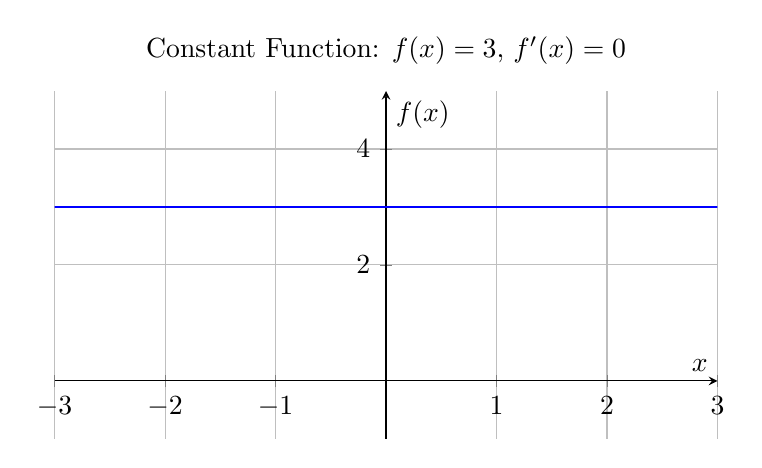
\begin{tikzpicture}
            \begin{axis}[
                axis lines = middle,
                xlabel = \(x\),
                ylabel = {\(f(x)\)},
                ymin=-1, ymax=5,
                xmin=-3, xmax=3,
                grid = major,
                width=10cm,
                height=6cm,
                title={Constant Function: \( f(x) = 3 \), \( f'(x) = 0 \)}
            ]
            \addplot[blue, thick] {3};
        \end{axis}
        \end{tikzpicture}
        \captionof{figure}{Graph of the constant function \( f(x) = 3 \). The slope of this function is zero everywhere, hence \( f'(x) = 0 \).}
    \end{center}

    \item \textbf{Sum Rule:} The derivative of the sum of functions is the sum of their derivatives.
    \begin{center}
        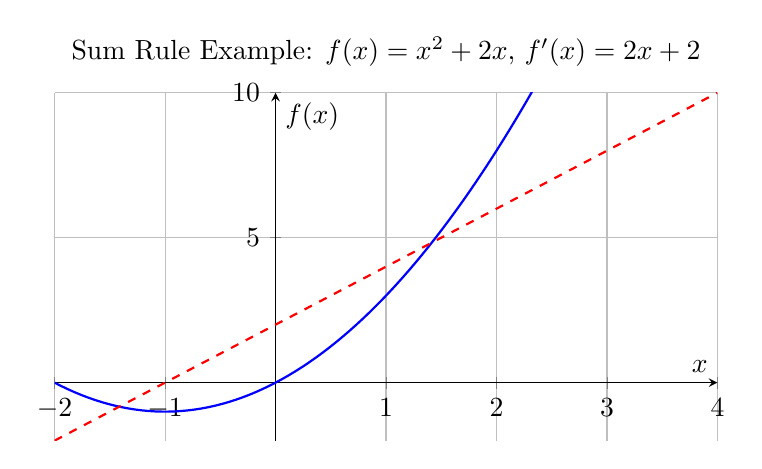
\begin{tikzpicture}
            \begin{axis}[
                axis lines = middle,
                xlabel = \(x\),
                ylabel = {\(f(x)\)},
                ymin=-2, ymax=10,
                xmin=-2, xmax=4,
                grid = major,
                width=10cm,
                height=6cm,
                domain=-2:4,
                samples=100,
                title={Sum Rule Example: \( f(x) = x^2 + 2x \), \( f'(x) = 2x + 2 \)}
            ]
            \addplot[blue, thick] {x^2 + 2*x};
            \addplot[red, dashed, thick] {2*x + 2};
        \end{axis}
        \end{tikzpicture}
        \captionof{figure}{Graph of \( f(x) = x^2 + 2x \) (blue) and its derivative \( f'(x) = 2x + 2 \) (red dashed). The derivative is the sum of the derivatives of \( x^2 \) and \( 2x \).}
    \end{center}

    \item \textbf{Product Rule:} If \( f(x) = g(x) \cdot h(x) \), then the derivative is \( f'(x) = g'(x)h(x) + g(x)h'(x) \).
    \begin{center}
        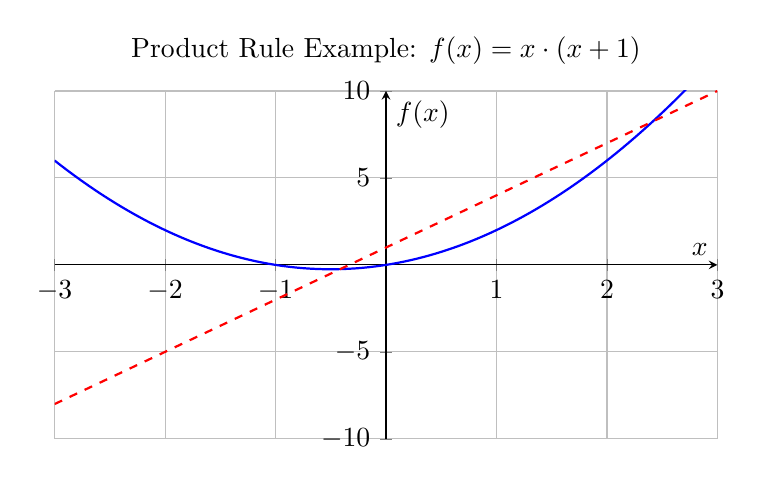
\begin{tikzpicture}
            \begin{axis}[
                axis lines = middle,
                xlabel = \(x\),
                ylabel = {\(f(x)\)},
                ymin=-10, ymax=10,
                xmin=-3, xmax=3,
                grid = major,
                width=10cm,
                height=6cm,
                domain=-3:3,
                samples=100,
                title={Product Rule Example: \( f(x) = x \cdot (x+1) \)}
            ]
            \addplot[blue, thick] {x * (x + 1)};
            \addplot[red, dashed, thick] {x + 2*x + 1};
        \end{axis}
        \end{tikzpicture}
        \captionof{figure}{Graph of the product function \( f(x) = x(x+1) \) (blue) and its derivative \( f'(x) = x + 2x + 1 \) (red dashed). The product rule combines the derivatives of both factors.}
    \end{center}
\end{itemize}


\begin{figure}[h!]
    \centering
    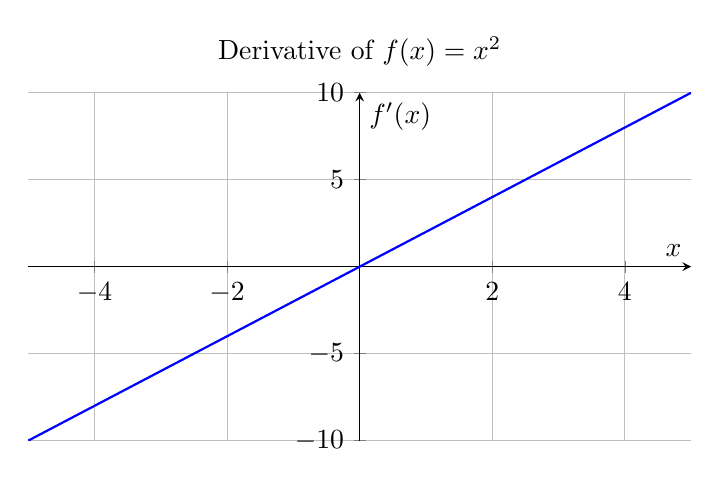
\begin{tikzpicture}
        \begin{axis}[
            axis lines = middle,
            xlabel = \(x\),
            ylabel = {\(f'(x)\)},
            ymin=-10, ymax=10,
            xmin=-5, xmax=5,
            grid = major,
            width=10cm,
            height=6cm,
            domain=-5:5,
            samples=100,
            title={Derivative of \( f(x) = x^2 \)}
        ]
        \addplot[blue, thick] {2*x};
    \end{axis}
    \end{tikzpicture}
    \caption{Graph of the derivative \( f'(x) = 2x \) of the function \( f(x) = x^2 \). The slope of \( f(x) \) changes depending on the value of \( x \).}
\end{figure}

In the examples above, the linear function \( f(x) = 2x + 3 \) has a constant rate of change of 2, which is the slope of the line. In contrast, the quadratic function \( f(x) = x^2 \) has a rate of change that varies depending on \( x \). The derivative \( f'(x) = 2x \) gives the slope of the tangent to the curve at any given point.


\subsection{Basic Rules for Derivatives}
\begin{enumerate}
    \item \textbf{Power Rule:} For any function of the form \( f(x) = x^n \), where \( n \) is a constant, the derivative is:
    \[
    f'(x) = n \cdot x^{n-1}
    \]
    \textbf{Example:}
    \begin{itemize}
        \item For \( f(x) = x^2 \), the derivative is: \( f'(x) = 2x \)
        \item For \( f(x) = x^3 \), the derivative is: \( f'(x) = 3x^2 \)
    \end{itemize}
    \item \textbf{Constant Rule:} The derivative of a constant is always 0. This is because a constant does not change, so its rate of change is 0.
    \textbf{Example:}
    \begin{itemize}
        \item For \( f(x) = 7 \), the derivative is \( f'(x) = 0 \).
    \end{itemize}
    \item \textbf{Sum and Difference Rule:} If you have two functions being added or subtracted, you can find the derivative of each part separately.
    \textbf{Example:}
    \begin{itemize}
        \item For \( f(x) = 3x^2 + 4x \), the derivative is: \( f'(x) = 6x + 4 \)
    \end{itemize}
\end{enumerate}

\subsection{Interpreting Derivatives}
The derivative gives you the slope of a curve at any point. If the slope is positive, the function is increasing at that point; if the slope is negative, the function is decreasing.

\section{Applications of Derivatives}
Derivatives are incredibly useful in real-world scenarios. Let’s look at a few practical examples:
\begin{enumerate}
    \item \textbf{Velocity:} If you know the position of an object as a function of time, the derivative of that function gives you the object’s velocity (rate of change of position).
    \textbf{Example:}
    \begin{itemize}
        \item If the position of a car over time is given by \( f(t) = t^2 \), the derivative, \( f'(t) = 2t \), tells us the car’s velocity at any time \( t \).
    \end{itemize}
    \item \textbf{Optimization:} Businesses use derivatives to find maximum profits or minimum costs. By taking the derivative of a profit or cost function, companies can determine when profits are at their highest or when costs are at their lowest.
    \item \textbf{Tangent Lines:} The derivative of a function at a point gives the slope of the tangent line to the curve at that point. A tangent line is a straight line that touches the curve at exactly one point and represents the best linear approximation of the curve near that point.
\end{enumerate}

\section{What Is an Integral?}
While derivatives focus on how things change, integrals help us calculate how much has accumulated over time. An integral measures the area under a curve.

Imagine you’re tracking the speed of a car over time. The integral of the speed function gives you the total distance the car has traveled.

\subsection{The Concept of Area}
In algebra, you can find the area of simple shapes like rectangles and triangles. In calculus, integrals allow you to find the area under curves, even if the shape is irregular.

\section{Finding Integrals}
Just like derivatives, there are rules for finding integrals. These rules help you calculate the total accumulation or area under a curve.

\subsection{Basic Rules for Integrals}
\begin{enumerate}
    \item \textbf{Power Rule for Integrals:} For any function of the form \( f(x) = x^n \), the integral is:
    \[
    \int x^n \, dx = \frac{x^{n+1}}{n+1} + C
    \]
    Where \( C \) is a constant (because integrals can have multiple solutions based on starting points).
    \textbf{Example:}
    \begin{itemize}
        \item For \( f(x) = x^2 \), the integral is: \( \int x^2 \, dx = \frac{x^3}{3} + C \)
    \end{itemize}
    \item \textbf{Constant Rule for Integrals:} The integral of a constant is the constant times \( x \).
    \textbf{Example:}
    \begin{itemize}
        \item For \( f(x) = 5 \), the integral is: \( \int 5 \, dx = 5x + C \)
    \end{itemize}
    \item \textbf{Sum and Difference Rule for Integrals:} You can integrate each part of a sum or difference separately.
    \textbf{Example:}
    \begin{itemize}
        \item For \( f(x) = 3x^2 + 2x \), the integral is: \( \int (3x^2 + 2x) \, dx = x^3 + x^2 + C \)
    \end{itemize}
\end{enumerate}

\section{Applications of Integrals}
Integrals have many practical applications, especially when you need to calculate totals, such as:
\begin{enumerate}
    \item \textbf{Area Under a Curve:} If you want to calculate the total area under a curve (for example, finding the total distance a car has traveled), integrals provide the solution.
    \textbf{Example:}
    \begin{itemize}
        \item If the velocity of a car is given by \( f(t) = 2t \), the integral of this function gives the distance traveled: \( \int 2t \, dt = t^2 + C \)
    \end{itemize}
    \item \textbf{Accumulating Quantities:} If you know how something is changing, you can use integrals to find the total amount accumulated over time. For example, if you know the rate at which water is flowing into a tank, you can use an integral to find the total amount of water in the tank after a certain time.
    \item \textbf{Economics and Finance:} Integrals are used in economics to calculate things like consumer surplus and producer surplus by finding the area under demand or supply curves.
\end{enumerate}

\section{Fundamental Theorem of Calculus}
The Fundamental Theorem of Calculus links derivatives and integrals. It states that:
\begin{enumerate}
    \item The derivative of the integral of a function is the function itself.
    \item The integral of the derivative of a function gives you the accumulated value of the function.
\end{enumerate}
In simple terms, derivatives and integrals are two sides of the same coin—one describes how something is changing, while the other describes how much has accumulated.

\section{Practice Makes Perfect: Let’s Try Some Exercises!}
\subsection{Derivatives}
\begin{enumerate}
    \item Find the derivative of \( f(x) = 4x^3 \).
    \item Find the derivative of \( f(x) = x^2 + 3x + 2 \).
\end{enumerate}

\subsection{Integrals}
\begin{enumerate}
    \item Find the integral of \( f(x) = x^2 \).
    \item Find the integral of \( f(x) = 3x + 5 \).
\end{enumerate}

\subsection{Applications}
\begin{enumerate}
    \item A car’s position is given by \( f(t) = t^2 + 2t \). Find the car’s velocity by taking the derivative.
    \item Find the area under the curve \( f(x) = 2x \) between \( x = 0 \) and \( x = 3 \).
\end{enumerate}

\section{Real-Life Applications of Calculus}
\begin{itemize}
    \item \textbf{Physics:} Calculus helps in understanding motion, forces, and energy. Derivatives are used to find velocities and accelerations, while integrals calculate distances and areas under curves.
    \item \textbf{Engineering:} Engineers use calculus to model systems that involve changes, such as heat flow, structural loads, and electrical circuits.
    \item \textbf{Medicine:} In pharmacokinetics, integrals help calculate the total amount of a drug in the bloodstream over time, while derivatives describe how quickly the drug is absorbed or eliminated.
\end{itemize}

\section{Chapter Summary}
\begin{itemize}
    \item Derivatives measure the rate of change of a function. They tell us how fast something is changing at a particular moment.
    \item Integrals measure accumulation. They help us calculate the total amount of something, such as the area under a curve.
    \item The Fundamental Theorem of Calculus connects derivatives and integrals, showing that they are inverse operations.
    \item Calculus has many real-world applications, from physics and engineering to economics and medicine.
\end{itemize}

\section{Challenge Question}
A car’s velocity is given by \( v(t) = 3t^2 \), where \( t \) is time in seconds. Find the car’s total distance traveled between \( t = 0 \) and \( t = 4 \) seconds by using an integral.